\documentclass[8pt]{beamer}
\usetheme{Madrid}
\usefonttheme{serif}

\usepackage{fontspec}
% надёжный шрифт с кириллицей (работает в Overleaf)
\setmainfont{Libertinus Serif}[Ligatures=TeX]
\setsansfont{Libertinus Sans}[Ligatures=TeX]
\newfontfamily\cyrillicfont{Libertinus Serif}
\newfontfamily\cyrillicfontsf{Libertinus Sans}
\usepackage{polyglossia}
\setmainlanguage{russian}
\setotherlanguage{english}

\usepackage{amsmath}
\usepackage{amsfonts}
\usepackage{amssymb}
\usepackage{graphicx}
\usepackage{microtype}

\usepackage{tabularx}
\usepackage{booktabs}

\usepackage{xcolor}
\usepackage{pifont}
\usepackage{tikz}
\newcommand{\plus}{\tikz[baseline=(X.base)] \node[fill=green!65!black, rounded corners=2pt, inner sep=2pt] (X) {\color{white}\ding{51}};}
\newcommand{\minus}{\tikz[baseline=(X.base)] \node[fill=red!70!black,   rounded corners=2pt, inner sep=2pt] (X) {\color{white}\ding{55}};}

\DeclareMathOperator{\sen}{sen}
% \DeclareMathOperator{\tg}{tg}

\setbeamertemplate{caption}[numbered]

% --- Информация о презентации ---
\author[Автор]{Чиняев Владимир Николаевич}
\title{Матрица перехода (state transition matrix) \\ Матрица возмущений \\ Универсальное решение задачи перехода}
\newcommand{\coursename}{Введение в маневрирование КА}
\setbeamertemplate{navigation symbols}{} 
\institute[]{Московский физико технический институт} 
\date{21 октября 2025 г.} 

\bibliographystyle{apalike}

% --- Кастомная нижняя синяя полоска: курс слева, номер слайда справа ---
\setbeamertemplate{footline}{
  \leavevmode%
  \begin{beamercolorbox}[wd=\paperwidth,ht=2ex,dp=1ex]{palette primary}
    \hspace{0.4cm}\usebeamerfont{footline}\coursename\hfill\usebeamerfont{footline}\insertframenumber\hspace{0.4cm}
  \end{beamercolorbox}%
}

% Чтобы убрать лишние отступы в footer-шрифте (опционально)
\setbeamerfont{footline}{size=\small}

\begin{document}

\begin{frame}
\titlepage
\end{frame}

\begin{frame}{Система уравнений движения в кеплеровых элементах}
\begin{equation*}
    \begin{aligned}
        \frac{da}{dt} &= \sqrt{\frac{p}{\mu}} \frac{2a}{1 - e^2} \left( S e \sin \nu + T \frac{p}{r} \right), \\
        \frac{de}{dt} &= \sqrt{\frac{p}{\mu}} \left\{ S \sin \nu + T \left[ \left(1 + \frac{r}{p} \right) \cos \nu + e \frac{r}{p} \right] \right\}, \\
        \frac{d \omega}{dt} &= \sqrt{\frac{p}{\mu}} \left\{ -S \frac{\cos \nu}{e} + T \frac{1}{e}  \left(1 + \frac{r}{p} \right) \sin \nu - W \frac{r}{p} \text{ctg } i \sin u  \right\}, \\
        \frac{d i}{dt} &= W \sqrt{\frac{p}{\mu}} \frac{r}{p} \cos u, \\
        \frac{d \Omega}{dt} &= W \sqrt{\frac{p}{\mu}} \frac{r}{p} \frac{\sin u}{\sin i}, \\
        \frac{d M}{dt} &= n + \sqrt{\frac{p}{\mu}} \frac{\sqrt{1 - e^2}}{e} \left\{ \left( \cos \nu - 2e \frac{r}{p} \right) S - \left(1 + \frac{r}{p} \right) \sin \nu T \right\}
    \end{aligned}
\end{equation*}
где 
\begin{equation*}
    r = \frac{p}{1 + e \cos \nu}, \quad p = a (1 - e^2), \quad u = \omega + \nu.
\end{equation*}
\begin{equation*}
    S = S(t), \; T = T(t), \; W = W(t) - \text{ непрерывные функции времени}.
\end{equation*}
\end{frame}

\begin{frame}{Система уравнений движения в кеплеровых элементах}
\begin{equation*}
    \dot{\mathbf{y}} = 
    \underbrace{
    \begin{bmatrix}
        0 \\ 0 \\ 0 \\ 0 \\ 0 \\ n(\mathbf{y})
    \end{bmatrix}
    }_{\mathbf{f}_\odot (\mathbf{y})}
    + 
    \underbrace{
    \begin{bmatrix}
        \sqrt{\frac{p}{\mu}} \frac{2a}{1 - e^2} e \sin \nu &
        \sqrt{\frac{p}{\mu}} \frac{2a}{1 - e^2} \frac{p}{r} & 
        0 \\

        \sqrt{\frac{p}{\mu}} \sin \nu &
        \sqrt{\frac{p}{\mu}} \left[ \left(1 + \frac{r}{p} \right) \cos \nu + e \frac{r}{p} \right] & 
        0 \\

        -\sqrt{\frac{p}{\mu}} \frac{\cos \nu}{e} &
        \sqrt{\frac{p}{\mu}} \frac{1}{e} \left(1 + \frac{r}{p} \right) \sin \nu &
        -\sqrt{\frac{p}{\mu}} \frac{r}{p} \text{ctg } i \sin u \\

        0 &
        0 &
        \sqrt{\frac{p}{\mu}} \frac{r}{p} \cos u \\

        0 & 
        0 &
        \sqrt{\frac{p}{\mu}} \frac{r}{p} \frac{\sin u}{\sin i} \\

        \sqrt{\frac{p}{\mu}} \frac{\sqrt{1 - e^2}}{e} \left( \cos \nu - 2e \frac{r}{p} \right) &
        -\sqrt{\frac{p}{\mu}} \frac{\sqrt{1 - e^2}}{e} \left(1 + \frac{r}{p} \right) \sin \nu &
        0
    \end{bmatrix}
    }_{B(\mathbf{y})}
    \underbrace{
    \begin{bmatrix}
        S \\ T \\ W
    \end{bmatrix}
    }_{\mathbf{a}}
\end{equation*}
\end{frame}

\begin{frame}{Импульсные манёвры}
\begin{columns}[T,totalwidth=\textwidth]
  % Левая колонка
  \begin{column}{0.49\textwidth}
    \begin{align*}
        &\dot{\mathbf{y}} = \mathbf{f}_\odot (\mathbf{y}) + B(\mathbf{y}) \mathbf{a}, \\
        &\mathbf{y} (t_0) = \mathbf{y}_0.
    \end{align*}
    Здесь 
    \begin{equation*}
        \mathbf{a} = c \; \mathbf{e} \; \theta(t), \quad \quad
        \theta(t) = 
        \begin{cases}
            1, t \in [t_0, t_1], \\
            0, t \notin [t_0, t_1].
        \end{cases}
    \end{equation*}
    $c = \text{const}$, $\mathbf{e}$ - постоянный единичный вектор. Таким образом $\mathbf{a}$ - простейшая модель протяжённого манёвра с постоянной ориентацией и модулем. 
  \end{column}

  % Правая колонка
  \begin{column}{0.49\textwidth}
    \begin{center}
        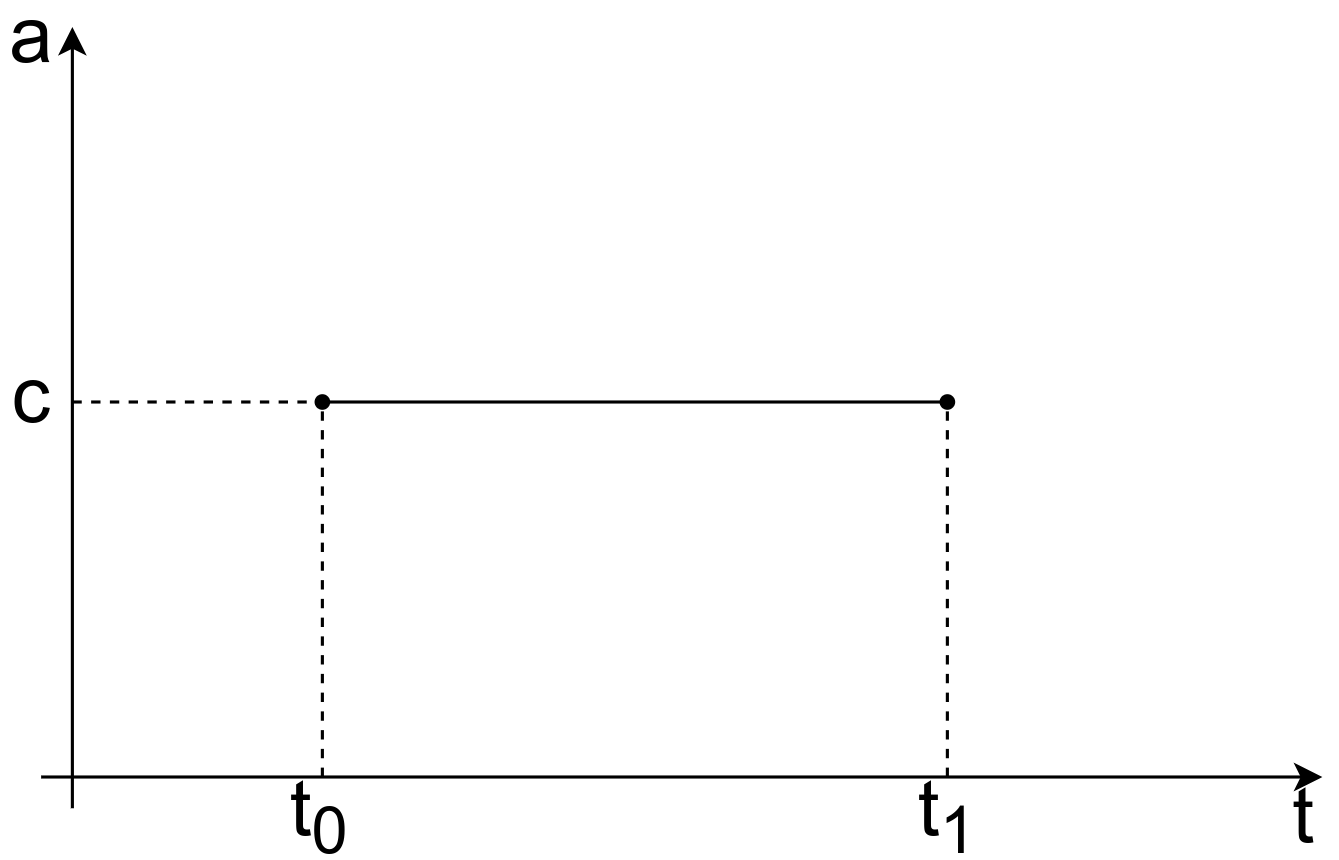
\includegraphics[height=0.40\textheight,keepaspectratio]{images/7/acc(t).png}
    \end{center}
  \end{column}
\end{columns}
\end{frame}

\begin{frame}{Импульсные манёвры}
\begin{align*}
    \Delta \mathbf{y} &= \int_{t_0}^{t_1} \mathbf{f}_\odot (\mathbf{y}) dt + \int_{t_0}^{t_1} B(\mathbf{y}) \mathbf{a} dt \approx \\
    &\approx \int_{t_0}^{t_1} \mathbf{f}_\odot (\mathbf{y}) dt + \int_{t_0}^{t_1} \left[ B(\mathbf{y}_0) + \frac{dB}{d \mathbf{y}} (\mathbf{y}_0) \delta \mathbf{y} + \frac{1}{2} \delta \mathbf{y}^\top \frac{d^2B}{d \mathbf{y}^2} (\mathbf{y}_0) \delta \mathbf{y} \right] \mathbf{a} dt = \\
    &= \int_{t_0}^{t_1} \mathbf{f}_\odot (\mathbf{y}) dt + \int_{t_0}^{t_1} \left[ B(\mathbf{y}_0) + \frac{dB}{d \mathbf{y}} (\mathbf{y}_0) \delta \mathbf{y} + \frac{1}{2} \delta \mathbf{y}^\top \frac{d^2B}{d \mathbf{y}^2} (\mathbf{y}_0) \delta \mathbf{y} \right] \frac{\Delta \mathbf{V}}{T} dt = \\
    &= \int_{t_0}^{t_1} \mathbf{f}_\odot (\mathbf{y}) dt + B(\mathbf{y}_0) \frac{\Delta \mathbf{V}}{T}  \int_{t_0}^{t_1} dt + \int_{t_0}^{t_1} \frac{dB}{d \mathbf{y}} (\mathbf{y}_0) \delta \mathbf{y} \frac{\Delta \mathbf{V}}{T} dt + \int_{t_0}^{t_1} \frac{1}{2} \delta \mathbf{y}^\top \frac{d^2B}{d \mathbf{y}^2} (\mathbf{y}_0) \delta \mathbf{y} \frac{\Delta \mathbf{V}}{T} dt = \\
    &= \int_{t_0}^{t_1} \mathbf{f}_\odot (\mathbf{y}) dt + B(\mathbf{y}_0) \Delta \mathbf{V} + \int_{t_0}^{t_1} \frac{dB}{d \mathbf{y}} (\mathbf{y}_0) \delta \mathbf{y} \frac{\Delta \mathbf{V}}{T} dt + \int_{t_0}^{t_1} \frac{1}{2} \delta \mathbf{y}^\top \frac{d^2B}{d \mathbf{y}^2} (\mathbf{y}_0) \delta \mathbf{y} \frac{\Delta \mathbf{V}}{T} dt.
\end{align*} 
\begin{columns}[T,totalwidth=\textwidth]
  % Левая колонка
  \begin{column}{0.49\textwidth}
    Здесь
    \begin{equation*}
        \mathbf{y} (t) = \mathbf{y}_0 + \delta \mathbf{y} (t).
    \end{equation*}
    Введём простейшую модель воздействия импульса на орбитальные элементы:
    \begin{equation*}
        \delta \mathbf{y} (t) = \mathbf{k} t,
    \end{equation*}
    где $\mathbf{k} \sim \frac{\Delta \mathbf{V}}{T} $ - постоянный вектор.
  \end{column}

  % Правая колонка
  \begin{column}{0.49\textwidth}
    \begin{center}
        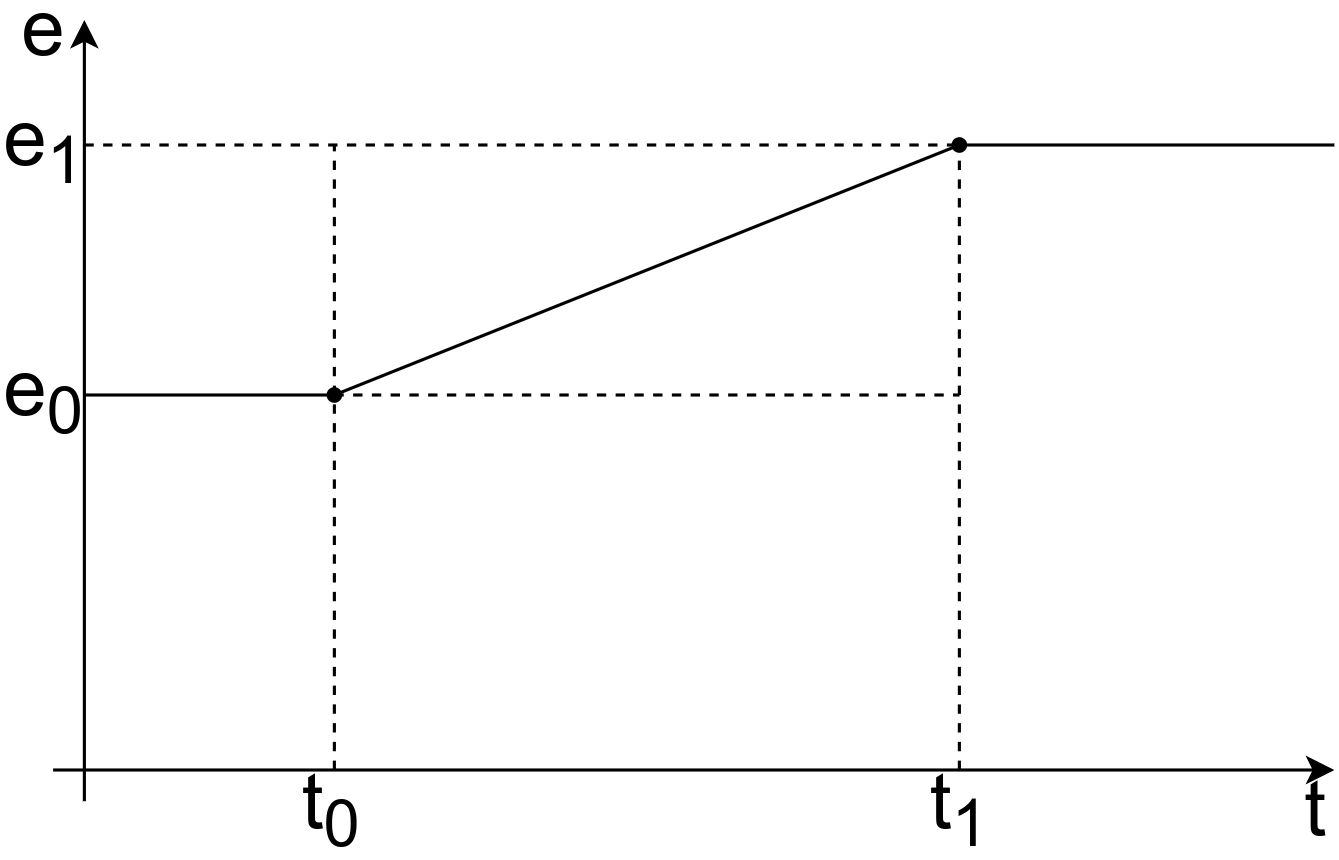
\includegraphics[height=0.30\textheight,keepaspectratio]{images/7/e(t).png}
    \end{center}
  \end{column}
\end{columns}
\end{frame}

\begin{frame}{Импульсные манёвры}
\begin{align*}
    \Delta \mathbf{y} &= \int_{t_0}^{t_1} \mathbf{f}_\odot (\mathbf{y}) dt + B(\mathbf{y}_0) \Delta \mathbf{V} + \int_{t_0}^{t_1} \frac{dB}{d \mathbf{y}} (\mathbf{y}_0) \delta \mathbf{y} \frac{\Delta \mathbf{V}}{T} dt + \int_{t_0}^{t_1} \frac{1}{2} \delta \mathbf{y}^\top \frac{d^2B}{d \mathbf{y}^2} (\mathbf{y}_0) \delta \mathbf{y} \frac{\Delta \mathbf{V}}{T} dt = \\
    &= \int_{t_0}^{t_1} \mathbf{f}_\odot (\mathbf{y}) dt + B(\mathbf{y}_0) \Delta \mathbf{V} + \frac{dB}{d \mathbf{y}} (\mathbf{y}_0) \mathbf{k}  \frac{\Delta \mathbf{V}}{T} \int_{t_0}^{t_1} t dt + \frac{1}{2} \mathbf{k}^\top \frac{d^2B}{d \mathbf{y}^2} (\mathbf{y}_0) \mathbf{k} \frac{\Delta \mathbf{V}}{T} \int_{t_0}^{t_1} t^2 dt = \\
    &= \int_{t_0}^{t_1} \mathbf{f}_\odot (\mathbf{y}) dt + B(\mathbf{y}_0) \Delta \mathbf{V} + O (|| \Delta \mathbf{V} ||^2).
\end{align*} 
Перейдём к пределу $T = | t_1 - t_0 | \longrightarrow 0$:
\begin{equation*}
    \boxed{
    \Delta \mathbf{y} = B(\mathbf{y}_0) \Delta \mathbf{V}
    }
\end{equation*}
Если величину хар. скорости некоторого манёвра по порядку оценить $|| \Delta \mathbf{V} || = 10~\text{м/с}$, то такое приближение даст относительную ошибку по хар. скорости порядка $\varepsilon \sim \frac{|| \Delta \mathbf{V} ||^2}{|| \mathbf{V} ||} = \frac{100}{7000} \sim 10^{-2}$.
\end{frame}

\begin{frame}{Импульсные манёвры}
\begin{center}
    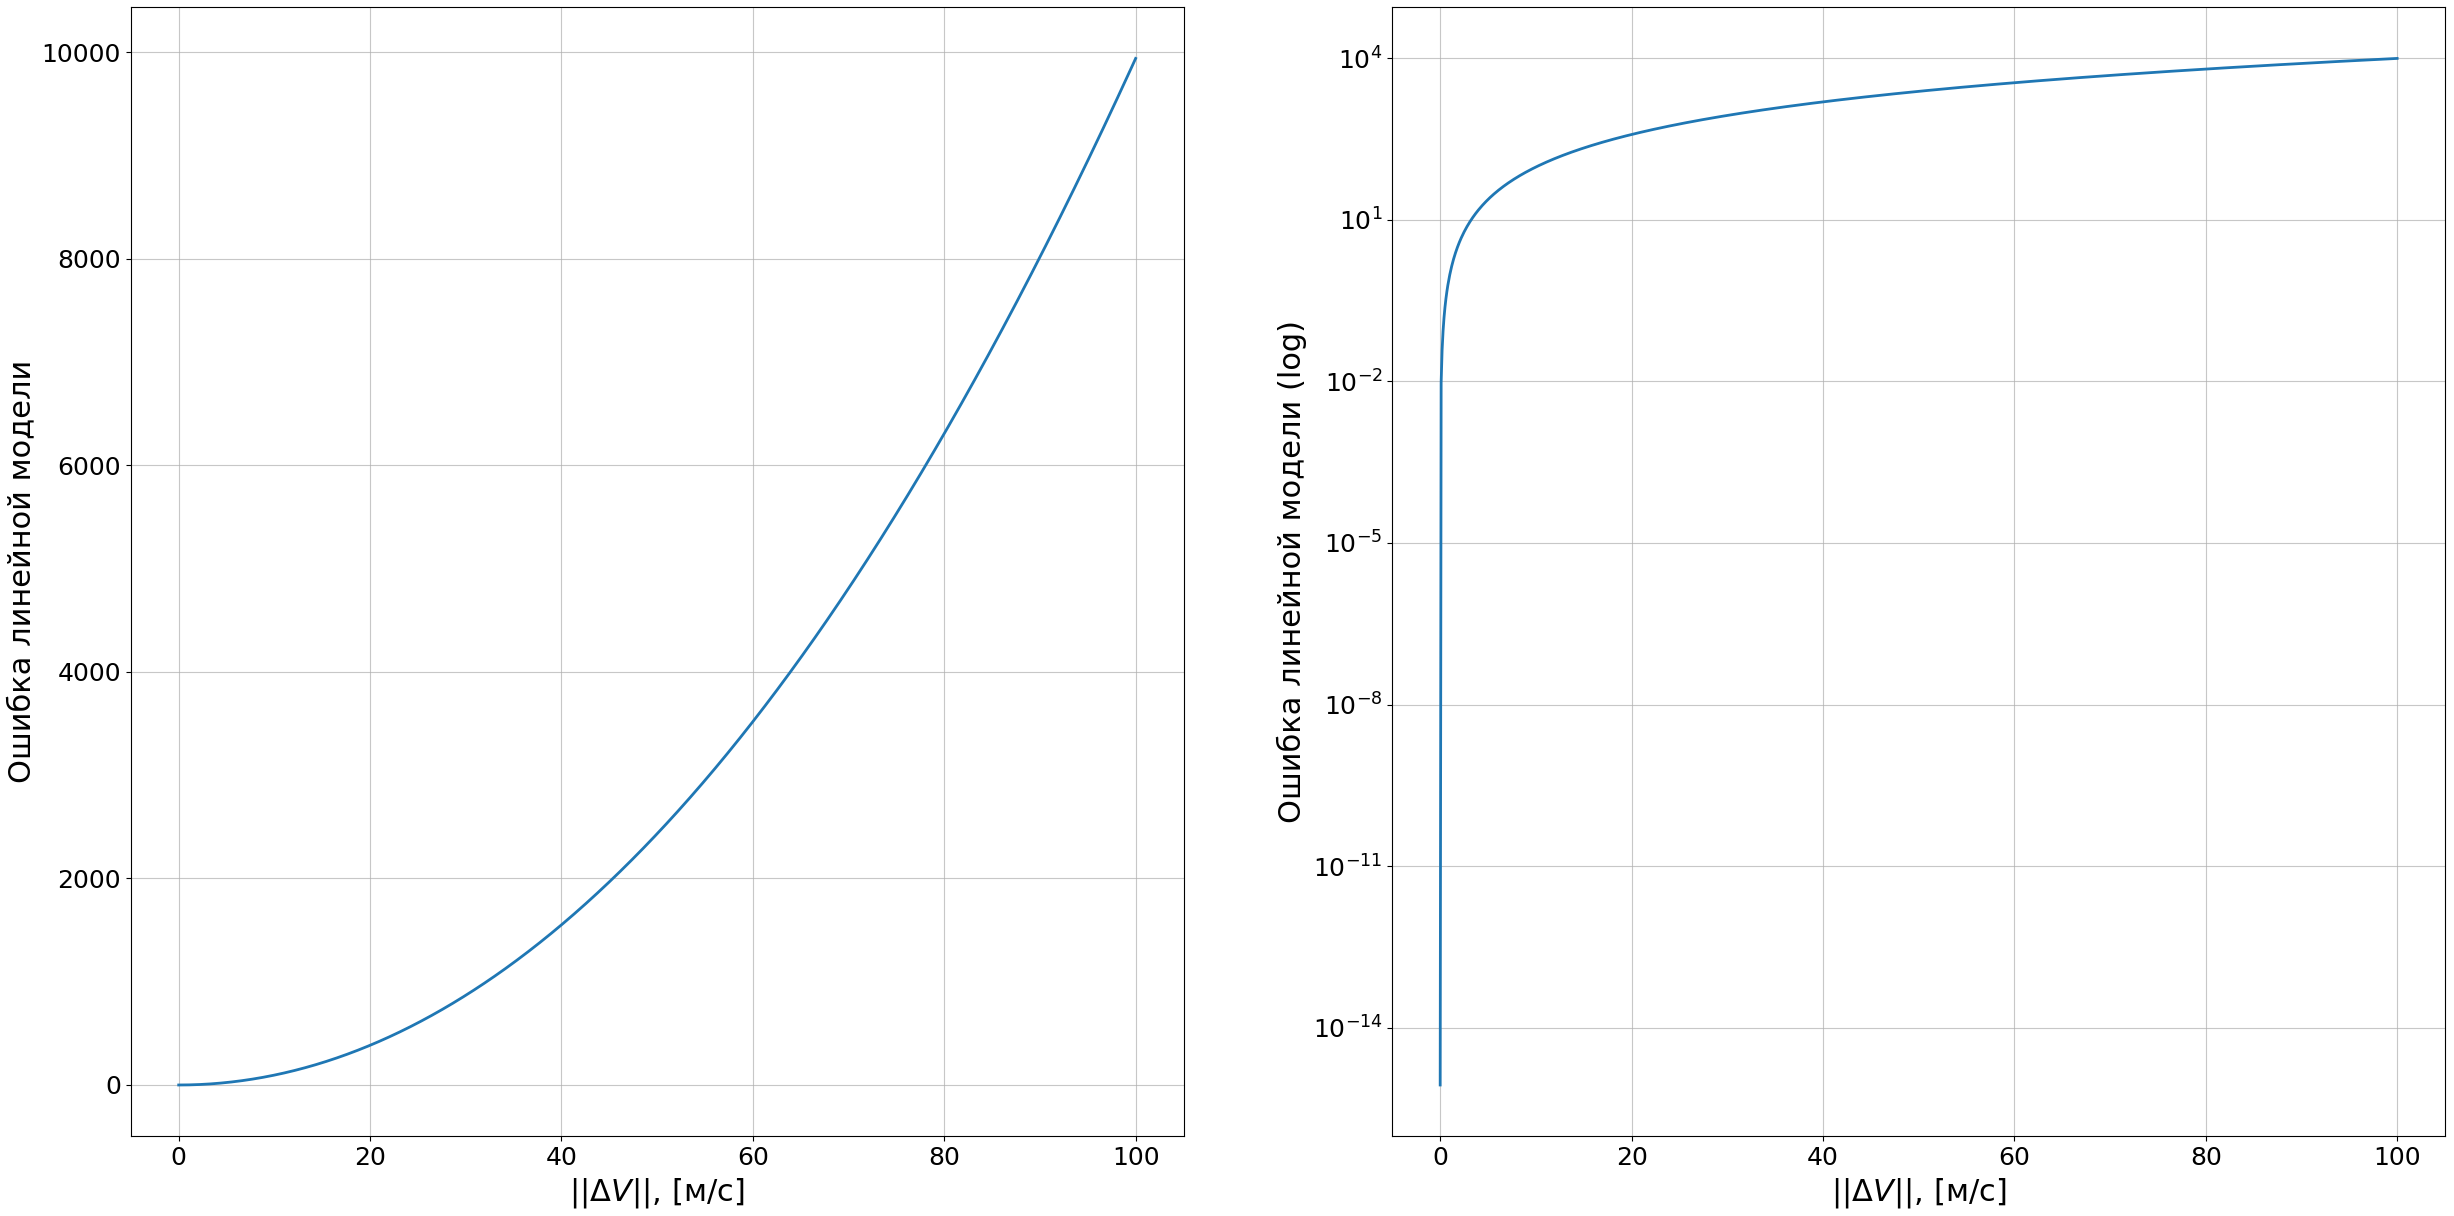
\includegraphics[height=0.65\textheight,keepaspectratio]{images/7/lin_model_error.png}
\end{center}
\end{frame}

\begin{frame}{Импульсные манёвры}
\begin{center}
    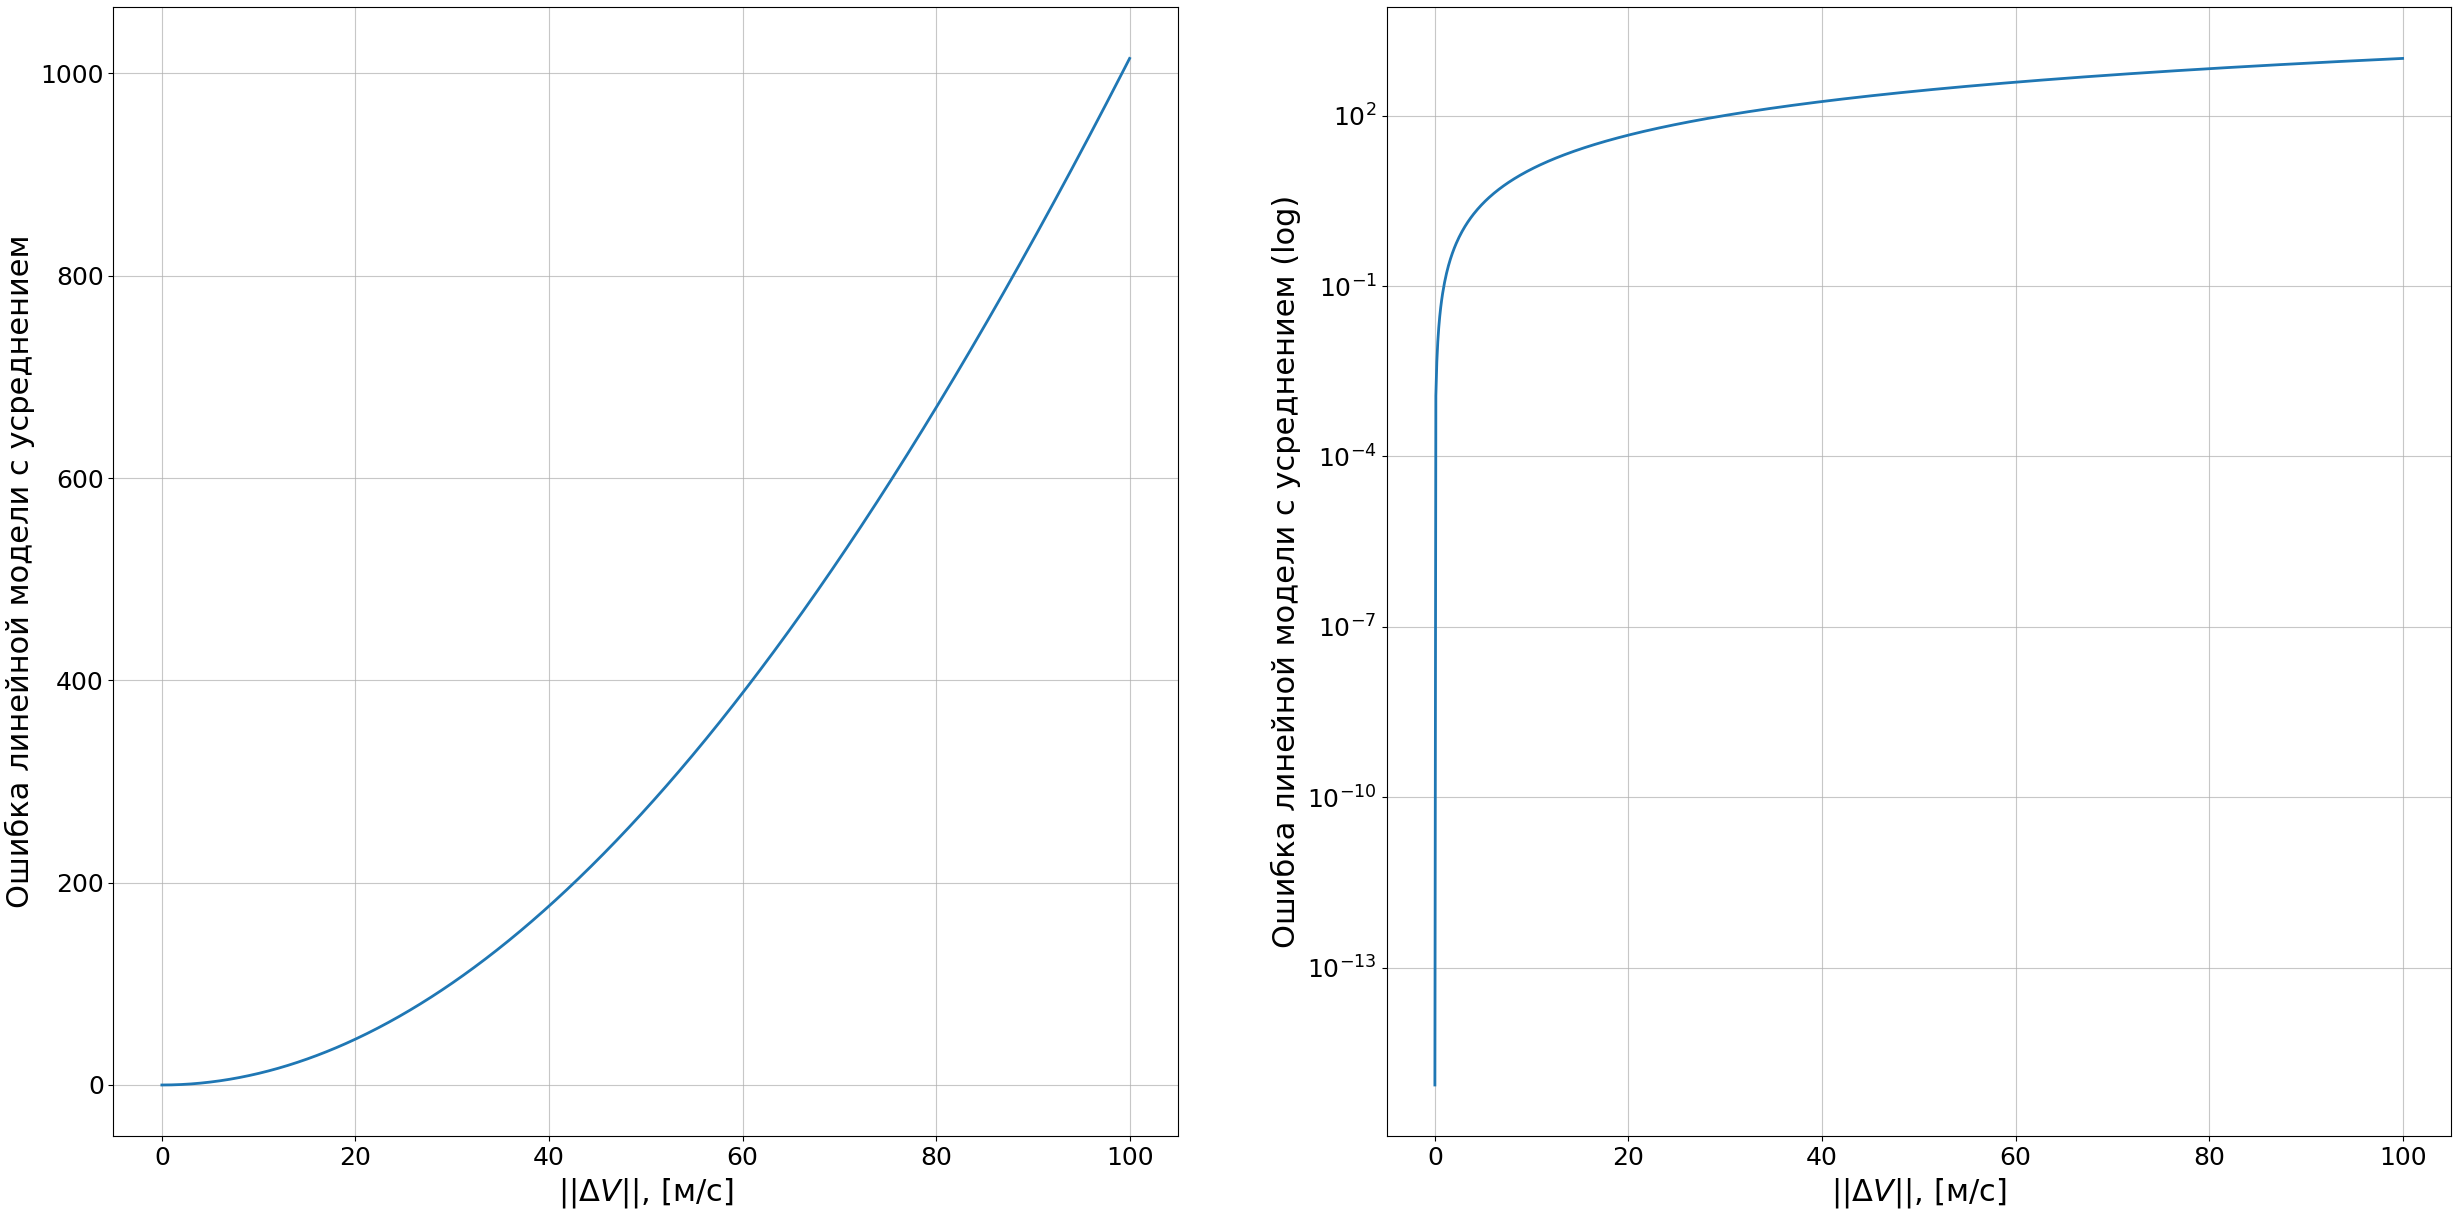
\includegraphics[height=0.65\textheight,keepaspectratio]{images/7/lin_model_error_2.png}
\end{center}
\end{frame}

\begin{frame}{Матрица перехода}
\begin{columns}[T,totalwidth=\textwidth]
  % Левая колонка
  \begin{column}{0.49\textwidth}
    \begin{center}
        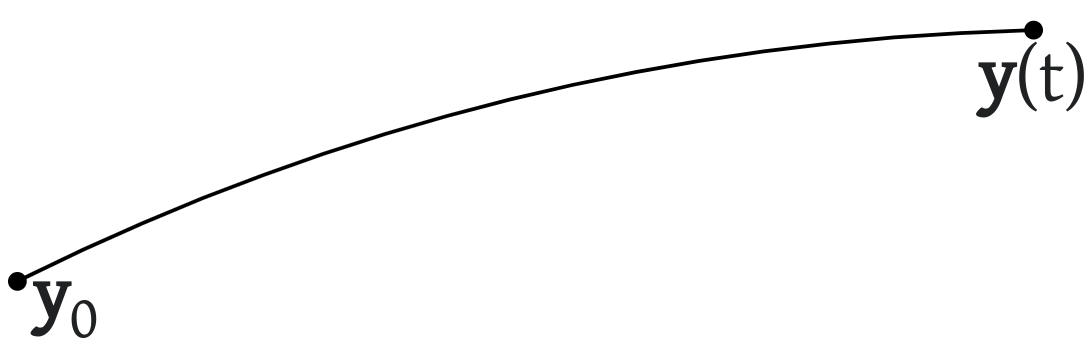
\includegraphics[height=0.20\textheight,keepaspectratio]{images/7/y0->y(t).png}
    \end{center}
    \textbf{Определение.} Матрица 
    \begin{equation*}
        \Phi = \frac{\partial \mathbf{y} (\mathbf{y}_0, t)}{\partial \mathbf{y}_0}.
    \end{equation*}
    называется \textbf{матрицей перехода} (state transition matrix, матрицей изохронных производных). Она показывает, как бесконечно малое изменение начального состояние повлияет на бесконечно малое изменение конечного состояния.  
  \end{column}

  % Правая колонка
  \begin{column}{0.49\textwidth}
  Вычислим $\Phi$, считая что КА движется в поле точечного потенциала. Тогда мы имеем начальное условие $\mathbf{y}_0$ и закон изменения элементов орбиты $\dot{\mathbf{y}}$:
    \begin{equation*}
        \mathbf{y}_0 = 
        \begin{bmatrix}
            a_0 \\ e_0 \\ \omega_0 \\ i_0 \\ \Omega_0 \\ M_0
        \end{bmatrix},
        \quad \quad
        \dot{\mathbf{y}} = 
        \begin{bmatrix}
            0 \\ 0 \\ 0 \\ 0 \\ 0 \\ n(a_0)
        \end{bmatrix}.
    \end{equation*}
    Состояние в произвольный момент времени $t$ может быть найдено точно:
    \begin{equation*}
        \mathbf{y}(t) = 
        \begin{bmatrix}
            a_0 \\ e_0 \\ \omega_0 \\ i_0 \\ \Omega_0 \\ M_0 + n(a_0) (t - t_0)
        \end{bmatrix}.
    \end{equation*}
  \end{column}
\end{columns}
\end{frame}

\begin{frame}{Матрица перехода}
Получим итоговое выражение:
\begin{align*}
    \Phi = \frac{\partial \mathbf{y}}{\partial \mathbf{y}_0} &= 
    \left[ \frac{\partial \mathbf{y}}{\partial a_0},
    \frac{\partial \mathbf{y}}{\partial e_0},
    \frac{\partial \mathbf{y}}{\partial \omega_0},
    \frac{\partial \mathbf{y}}{\partial i_0}, 
    \frac{\partial \mathbf{y}}{\partial \Omega_0}, 
    \frac{\partial \mathbf{y}}{\partial M_0}\right] = \\
    &=
    \begin{bmatrix}
        1 & 0 & 0 & 0 & 0 & 0 \\
        0 & 1 & 0 & 0 & 0 & 0 \\
        0 & 0 & 1 & 0 & 0 & 0 \\
        0 & 0 & 0 & 1 & 0 & 0 \\
        0 & 0 & 0 & 0 & 1 & 0 \\
        -\frac{3}{2} \frac{n}{a} (t - t_0) & 0 & 0 & 0 & 0 & 1 \\
    \end{bmatrix}.
\end{align*}
Важно отметить, выражение для $\Phi$ является \textbf{точным}.
\end{frame}

\begin{frame}{Матрица манёвра}
\begin{columns}[T,totalwidth=\textwidth]
  % Левая колонка
  \begin{column}{0.49\textwidth}
    \begin{center}
        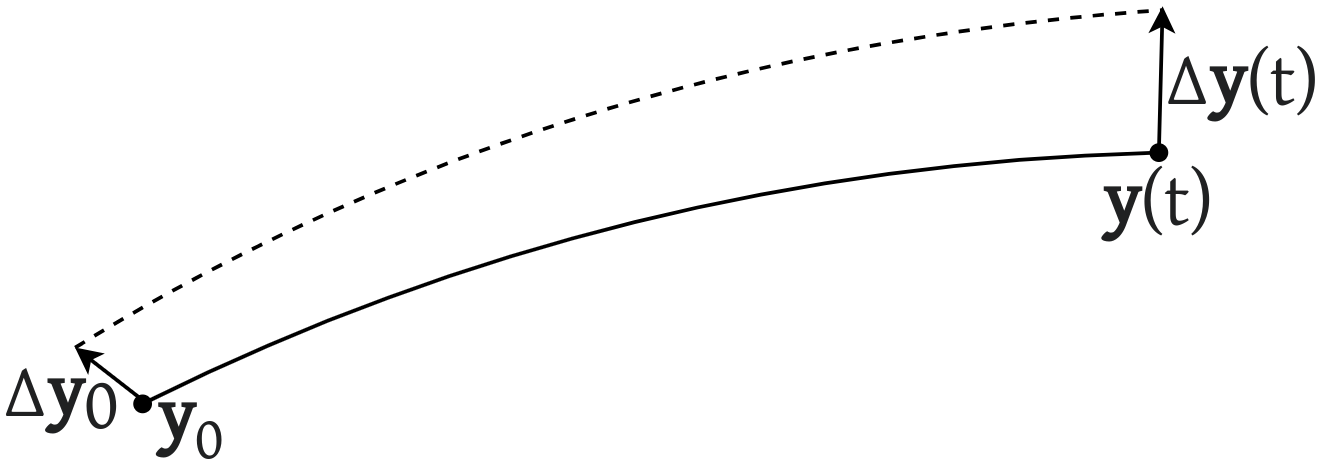
\includegraphics[height=0.20\textheight,keepaspectratio]{images/7/dy0->dy(t).png}
    \end{center}
    \begin{align*}
        \Delta \mathbf{y}(t) &= \frac{\partial \mathbf{y}}{\partial \mathbf{y}_0} (\mathbf{y}_0, t) \Delta \mathbf{y}_0 = \\
        &= \frac{\partial \mathbf{y}}{\partial \mathbf{y}_0} (\mathbf{y}_0, t) B(\mathbf{y}_0) \Delta \mathbf{V} = \\
        &= M (\mathbf{y}_0, t) \Delta \mathbf{V}.
    \end{align*}
    \textbf{Определение.} Мы будем называть матрицу 
    \begin{equation*}
        M (\mathbf{y}_0, t) = \frac{\partial \mathbf{y}}{\partial \mathbf{y}_0} (\mathbf{y}_0, t) B(\mathbf{y}_0)
    \end{equation*}
    \textbf{матрицей манёвра}. Она показывает, как мгновенное возмущение $\Delta \mathbf{V}$ в начальный момент времени $t_0$ повлияет на изменение орбитальных элементов в рассматриваемый момент времени $t$. 
  \end{column}

  % Правая колонка 
  \begin{column}{0.49\textwidth}
    Оценим ошибку. Она будет определяться первым отброшенным слагаемым:
    \begin{equation*}
        \varepsilon \sim \frac{1}{2} \Delta \mathbf{y}_0^\top \frac{\partial^2 \mathbf{y}}{\partial^2 \mathbf{y}_0} (\mathbf{y}_0, t) \Delta \mathbf{y}_0.
    \end{equation*}
    Если $\Delta \mathbf{y}_0$ имел ошибку $\sim 10^{-2}$, то $\Delta \mathbf{y}$ будет иметь относительную ошибку $\sim 10^{-4}$.
  \end{column}
\end{columns}
\end{frame}

\begin{frame}{Задача перехода}
\begin{columns}[T,totalwidth=\textwidth]
  % Левая колонка
  \begin{column}{0.49\textwidth}
    Рассмотрим такую модель:
    \begin{equation*}
        M_1 \Delta V_1 + M_2 \Delta V_2 = \Delta \mathbf{y}.
    \end{equation*}
    где
    \begin{itemize}
        \item $M_1 = M (\mathbf{y}(t_1), t_f) \in \mathbb{R}^{5 \times 3}$;
        \item $M_2 = M (\mathbf{y}(t_2), t_f) \in \mathbb{R}^{5 \times 2}$;
        \item $\Delta V_1, \Delta V_2 \in \mathbb{R}^{3 \times 1}$;
        \item $\Delta y = [\Delta a, \; \Delta e, \; \Delta \omega, \; \Delta i, \; \Delta \Omega]^\top \in \mathbb{R}^{5 \times 1}$.
    \end{itemize}
    Перепишем это выражение:
    \begin{equation*}
        M \Delta V = \Delta \mathbf{y},
    \end{equation*}
    где 
    \begin{equation*}
        M = 
        \begin{bmatrix}
            M_1 & M_2
        \end{bmatrix}
        \in \mathbb{R}^{5 \times 5},
    \end{equation*}
    \begin{equation*}
        \Delta V = 
        \begin{bmatrix}
            \Delta V_1 \\ \Delta V_2
        \end{bmatrix}
        \in \mathbb{R}^{5 \times 1}.
    \end{equation*}
  \end{column}

  % Правая колонка 
  \begin{column}{0.49\textwidth}
    \begin{center}
        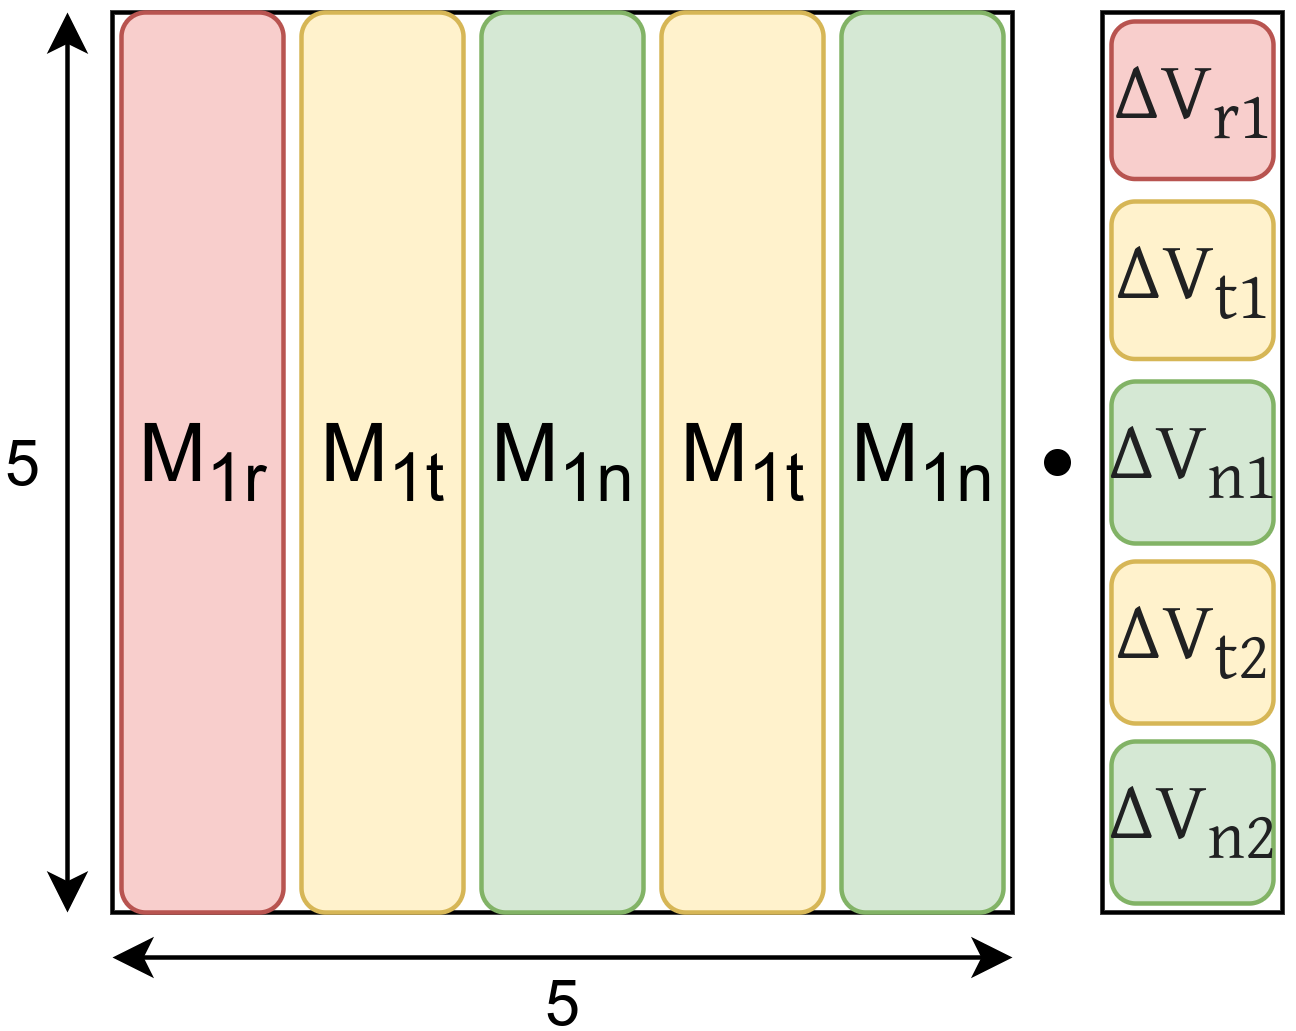
\includegraphics[height=0.50\textheight,keepaspectratio]{images/7/MV.png}
    \end{center}
  \end{column}
\end{columns}
\end{frame}

\begin{frame}{Задача перехода}
\begin{columns}[T,totalwidth=\textwidth]
  % Левая колонка
  \begin{column}{0.49\textwidth}
    \textbf{Дано:} 
    \begin{itemize}
        \item Начальная точка $\mathbf{y}(t_0)$;
        \item Точки приложения манёвров: $\mathbf{y}(t_1), \mathbf{y}(t_2)$;
        \item Целевая орбита $\mathbf{y}_t$;
        \item Точность выхода на целевую орбиту $\varepsilon$.
    \end{itemize}
    \textbf{Найти:}
    \begin{itemize}
        \item $\Delta V_1, \Delta V_2$. 
    \end{itemize}
    \textbf{Решение:}
    \begin{enumerate}
        \item $\mathbf{y}(t_1) \longrightarrow M_1$;
        \item $\mathbf{y}(t_2) \longrightarrow M_2$;
        \item Получить пассивный прогноз $\mathbf{y}_{\text{пас}}(t_f)$;
        \item $\epsilon = \text{dist}(\mathbf{y}_t, \mathbf{y}_{\text{пас}}(t_f))$;
        \item Повторять пока $\epsilon > \varepsilon$:
            \begin{align*}
                &\text{Сделать активный прогноз } \mathbf{y}(t_f) \\
                &\epsilon = \text{dist}(\mathbf{y}_t, \mathbf{y}(t_f)) \\
                &\Delta \mathbf{y} = \mathbf{y}_t - \mathbf{y}(t_f) \\
                &M \Delta V = \Delta \mathbf{y} \longrightarrow \Delta V
            \end{align*}
    \end{enumerate}
  \end{column}

  % Правая колонка 
  \begin{column}{0.49\textwidth}
    \begin{center}
        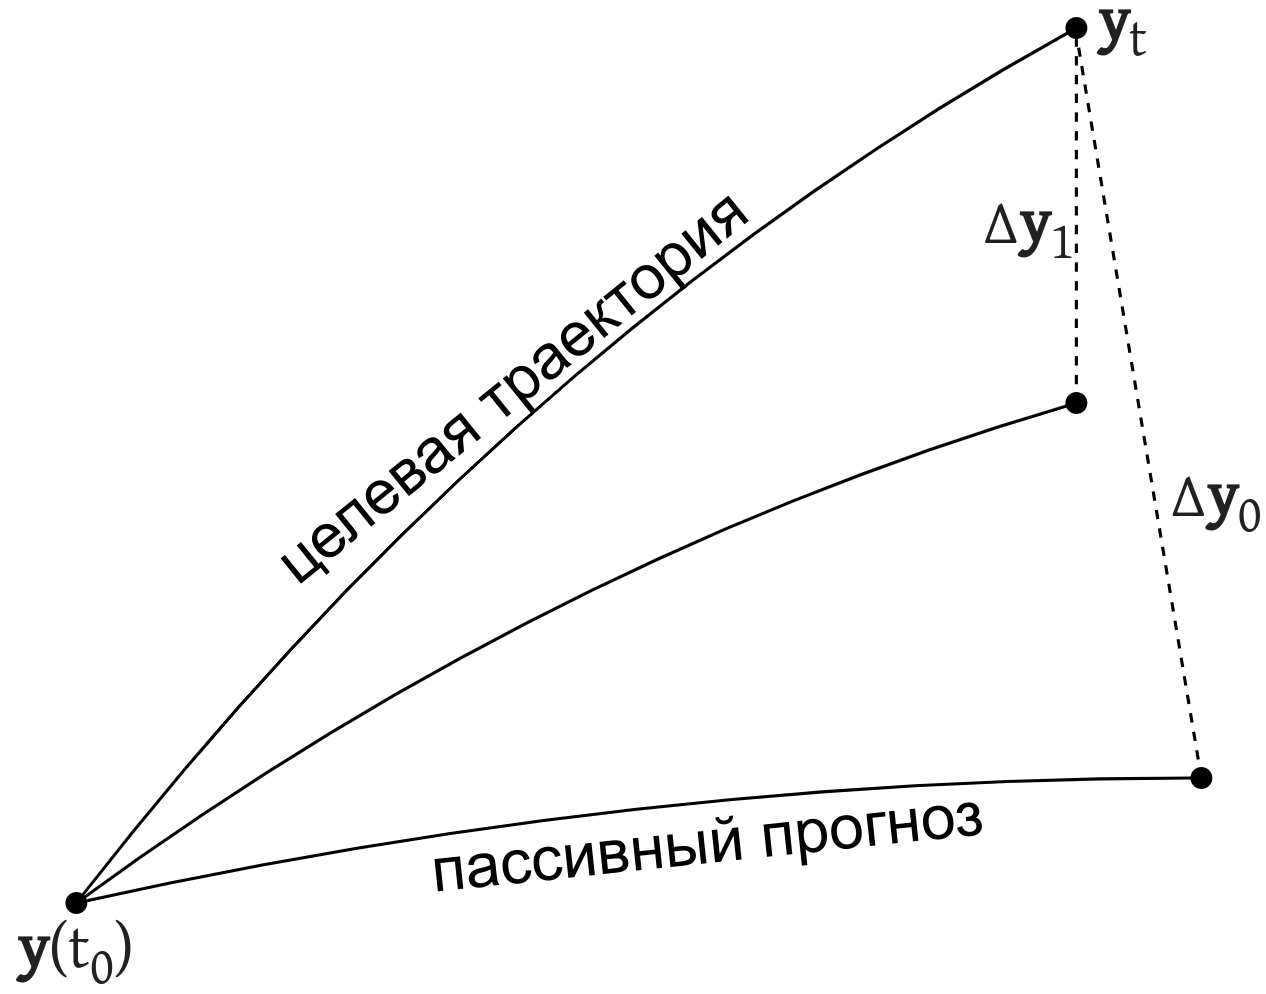
\includegraphics[height=0.50\textheight,keepaspectratio]{images/7/y(t).png}
    \end{center}
  \end{column}
\end{columns}
\end{frame}

\begin{frame}[allowframebreaks]{Источники}
  \begin{thebibliography}{9}

    \bibitem{Eliasberg}
    Эльясберг П. Е. Введение в теорию полета искусственных спутников Земли. – 1965.

    \bibitem{Vallado}
    Vallado D. A. Fundamentals of astrodynamics and applications. – Springer Science \& Business Media, 2001. – Т. 12.

    \bibitem{Baranov}
    Баранов А. А. Маневрирование космических аппаратов в окрестности круговой орбиты //М.: Спутник. – 2016.
    
  \end{thebibliography}
\end{frame}

\end{document}
